\documentclass[11pt,a4paper]{article}
\usepackage[utf8]{inputenc}
\usepackage[margin=2.2cm]{geometry}
\usepackage{booktabs}
\usepackage{forest}
\usepackage{tikz}
\usetikzlibrary{arrows.meta,positioning}
\usepackage{pdflscape}
\title{SafeSlice, Step 3: Ontology Design\\ \large Class trees, relations, and the full picture}
\author{SafeSlice group}
\date{v1.0}
\begin{document}
\maketitle
\noindent How to read the diagrams: tree arrows mean "is a kind of" (subclass). In the relation diagram and the one picture view, solid arrows are typed properties and dashed arrows are derived relations that the reasoner or the datalog engine must produce. Nobody ever types a contains fact by hand, that is the whole point of the project.

\section{Ontology overview (top level)}

\begin{center}
\begin{forest}
for tree={draw, rounded corners, font=\small, edge={-latex},
  l sep=8mm, s sep=3mm, align=center}
[owl:Thing
  [Pizza]
  [Ingredient]
  [DoughBase]
  [DietaryRestriction]
  [Customer]
  [Certification]
  [SpicinessLevel]
]
\end{forest}
\end{center}

\section{Class trees per branch}

\subsection{DietaryRestriction}
\begin{center}
\begin{forest}
for tree={draw, rounded corners, font=\footnotesize, edge={-latex}, l sep=7mm, s sep=1.6mm}
[DietaryRestriction
  [Diet
    [VeganDiet][VegetarianDiet][PescatarianDiet][HalalDiet][KosherDiet]
  ]
  [Allergy
    [NutAllergy][GlutenIntolerance][LactoseIntolerance]
  ]
]
\end{forest}
\end{center}

\subsection{DoughBase and SpicinessLevel}
\begin{center}
\begin{forest} for tree={draw, rounded corners, font=\small, edge={-latex}, l sep=7mm, s sep=3mm}
[DoughBase [NormalDough][GlutenFreeDough][VeganDough]]
\end{forest}
\qquad
\begin{forest} for tree={draw, rounded corners, font=\small, edge={-latex}, l sep=7mm, s sep=3mm}
[SpicinessLevel [NotSpicy][MediumSpicy][HotSpicy]]
\end{forest}
\end{center}
\noindent\emph{SpicinessLevel is a value partition: the three levels are pairwise disjoint and cover the class.}

\subsection{Pizza (named pizzas as subclasses)}
\begin{center}
\begin{forest}
for tree={draw, rounded corners, font=\footnotesize, edge={-latex},
  l sep=7mm, s sep=1.6mm, grow'=0, child anchor=west, parent anchor=east, anchor=west, tier/.option=level}
[Pizza
 [MargheritaPizza][PepperoniPizza][QuattroFormaggiPizza][HawaiianPizza][VegetarianaPizza]
 [PestoSpecialePizza][TonnoPizza][VeganGardenPizza][DiavolaPizza][FunghiPizza]
]
\end{forest}
\end{center}

\subsection{Ingredient (the large branch)}
\begin{center}
\begin{forest}
for tree={draw, rounded corners, font=\footnotesize, edge={-latex},
  grow'=0, child anchor=west, parent anchor=east, anchor=west,
  l sep=6mm, s sep=1.1mm, tier/.option=level}
[Ingredient
  [Vegetable
    [Tomato][Onion][Olive][Rucola][Garlic]
    [Herb [Basil][Oregano]]
    [PepperVegetable [BellPepper][Jalapeno]]
  ]
  [Cheese [Mozzarella][Parmesan][Gorgonzola][Provola][VeganCheese]]
  [Meat [Ham][Salami][Pepperoni][Chicken][PorkGelatin]]
  [Fish [Tuna][Anchovy]]
  [Fruit [Pineapple]]
  [Fungus [Mushroom]]
  [Nut [PineNut]]
  [Sauce [TomatoSauce][Pesto][GarlicOil]]
  [Spice [BlackPepper][ChiliFlakes]]
  [BaseIngredient [WheatFlour][GlutenFreeFlour][Water][Yeast][Salt][OliveOil][Egg]]
  [Component [Gluten][Milk][Pork]]
]
\end{forest}
\end{center}

\section{Relations (properties) and how classes connect}

\begin{center}
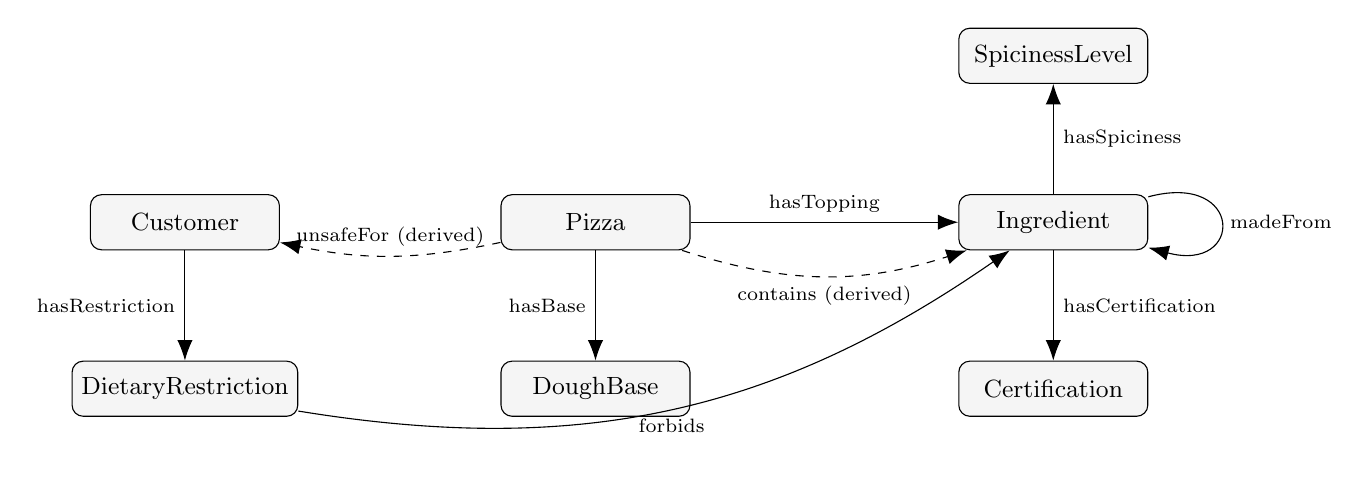
\begin{tikzpicture}[
  node distance=14mm and 20mm,
  box/.style={draw, rounded corners, fill=gray!8, minimum height=7mm, minimum width=24mm, font=\small},
  rel/.style={-{Latex[length=2.6mm]}, font=\scriptsize},
  der/.style={-{Latex[length=2.6mm]}, dashed, font=\scriptsize}
]
\node[box] (pizza) {Pizza};
\node[box, right=34mm of pizza] (ing) {Ingredient};
\node[box, below=of pizza] (base) {DoughBase};
\node[box, below=of ing] (cert) {Certification};
\node[box, left=28mm of pizza] (cust) {Customer};
\node[box, below=of cust] (res) {DietaryRestriction};
\node[box, above=of ing] (spice) {SpicinessLevel};

\draw[rel] (pizza) -- node[above]{hasTopping} (ing);
\draw[rel] (pizza) -- node[left]{hasBase} (base);
\draw[rel] (ing) edge[loop right, looseness=5] node[right]{madeFrom} (ing);
\draw[der] (pizza) to[bend right=18] node[below]{contains (derived)} (ing);
\draw[rel] (cust) -- node[left]{hasRestriction} (res);
\draw[rel] (res) to[bend right=22] node[below]{forbids} (ing);
\draw[rel] (ing) -- node[right]{hasCertification} (cert);
\draw[rel] (ing) -- node[right]{hasSpiciness} (spice);
\draw[der] (pizza) to[bend left=12] node[above]{unsafeFor (derived)} (cust);
\end{tikzpicture}
\end{center}

\begin{table}[h]\centering\small
\begin{tabular}{lll}
\toprule
\textbf{Property} & \textbf{Signature} & \textbf{Typed or derived}\\
\midrule
hasTopping & Pizza $\to$ Ingredient & typed (data/pizzas.csv)\\
hasBase & Pizza $\to$ DoughBase & typed (data/bases.csv)\\
madeFrom & Ingredient $\to$ Ingredient & typed (data/madefrom.csv)\\
contains & Pizza $\to$ Ingredient & \textbf{derived} (chains)\\
hasSpiciness & Ingredient $\to$ SpicinessLevel & typed\\
hasRestriction & Customer $\to$ DietaryRestriction & typed (data/customers.csv)\\
forbids & DietaryRestriction $\to$ category & typed (data/restrictions.csv)\\
hasCertification & Ingredient $\to$ Certification & typed\\
unsafeFor & Pizza $\to$ Customer & \textbf{derived}\\
safeFor & Pizza $\to$ Customer & \textbf{derived} (negation)\\
\bottomrule
\end{tabular}
\caption{All properties. Derived relations must come from the reasoner/engine, never typed in.}
\end{table}

\begin{landscape}
\section{The whole ontology in one picture}
\noindent Legend: \textbf{solid black arrows} = subclass (is-a) hierarchy; \textcolor{blue}{\textbf{blue arrows}} = typed properties; \textcolor{red}{\textbf{red dashed arrows}} = derived relations (the reasoner/engine must produce these).
\begin{center}
\resizebox{!}{0.9\textheight}{%
\begin{forest}
for tree={draw, rounded corners, font=\scriptsize, edge={-latex},
  grow'=0, child anchor=west, parent anchor=east, anchor=west,
  l sep=4.5mm, s sep=0.55mm, inner sep=1.1pt, tier/.option=level}
[owl:Thing
  [Customer, name=cust
    [\textit{anna, omar, mia, lisa, tom}, draw=gray, dashed]
  ]
  [DietaryRestriction, name=res
    [Diet [VeganDiet][VegetarianDiet][PescatarianDiet][HalalDiet][KosherDiet]]
    [Allergy [NutAllergy][GlutenIntolerance][LactoseIntolerance]]
  ]
  [Pizza, name=pizza
    [MargheritaPizza][PepperoniPizza][QuattroFormaggiPizza][HawaiianPizza][VegetarianaPizza]
    [PestoSpecialePizza][TonnoPizza][VeganGardenPizza][DiavolaPizza][FunghiPizza]
  ]
  [DoughBase, name=base [NormalDough][GlutenFreeDough][VeganDough]]
  [Ingredient, name=ing
    [Vegetable [Tomato][Onion][Olive][Rucola][Garlic]
      [Herb [Basil][Oregano]]
      [PepperVegetable [BellPepper][Jalapeno, name=jala]]
    ]
    [Cheese [Mozzarella][Parmesan][Gorgonzola][Provola][VeganCheese]]
    [Meat [Ham][Salami][Pepperoni][Chicken][PorkGelatin, name=gel]]
    [Fish [Tuna][Anchovy]]
    [Fruit [Pineapple]]
    [Fungus [Mushroom]]
    [Nut [PineNut]]
    [Sauce [TomatoSauce][Pesto][GarlicOil]]
    [Spice [BlackPepper][ChiliFlakes]]
    [BaseIngredient [WheatFlour][GlutenFreeFlour][Water][Yeast][Salt][OliveOil][Egg]]
    [Component [Gluten][Milk][Pork]]
  ]
  [Certification, name=cert [HalalCertified][KosherCertified][VeganCertified]]
  [SpicinessLevel, name=spice [NotSpicy][MediumSpicy][HotSpicy]]
]
% property arrows between branch anchors
\draw[-latex, blue, thick] (pizza.south) to[bend right=12] node[font=\scriptsize, fill=white, inner sep=1pt]{hasTopping} (ing.west);
\draw[-latex, blue, thick] (pizza.north) to[bend left=10] node[font=\scriptsize, fill=white, inner sep=1pt]{hasBase} (base.west);
\draw[-latex, blue, thick] (ing.south east) to[loop, looseness=3, in=-60, out=-20] node[font=\scriptsize, fill=white, inner sep=1pt]{madeFrom} (ing.east);
\draw[-latex, blue, thick] (cust.east) to[bend left=8] node[font=\scriptsize, fill=white, inner sep=1pt]{hasRestriction} (res.west);
\draw[-latex, blue, thick] (res.south) to[bend right=20] node[font=\scriptsize, fill=white, inner sep=1pt]{forbids} (ing.north west);
\draw[-latex, blue, thick] (gel.east) to[bend left=35] node[font=\scriptsize, fill=white, inner sep=1pt]{hasCertification} (cert.west);
\draw[-latex, blue, thick] (jala.east) to[bend left=55] node[font=\scriptsize, fill=white, inner sep=1pt]{hasSpiciness} (spice.west);
\draw[-latex, red, dashed, thick] (pizza.east) to[bend left=18] node[font=\scriptsize, fill=white, inner sep=1pt]{contains (derived)} (ing.north);
\draw[-latex, red, dashed, thick] (pizza.west) to[bend right=15] node[font=\scriptsize, fill=white, inner sep=1pt]{unsafeFor / safeFor (derived)} (cust.south);
\end{forest}}%
\end{center}
\end{landscape}
\end{document}
